\subsection{Introduction}
As already stated in the previous chapters, it is well-known that in general the electrophysiological
signal (acquired from a single electrode) is characterized by 2 distinct patterns:
\begin{itemize}
    \item \textbf{Spike:} a single over-threshold signal representing the activity of one or
          more neurons (typically a so-called unit or channel).
    \item \textbf{Burst:} a sequence of highly packed spikes often occurring simultaneously on
          several channels and giving rise to a phenomenon known as network burst.
\end{itemize}
\begin{figure}[H]
    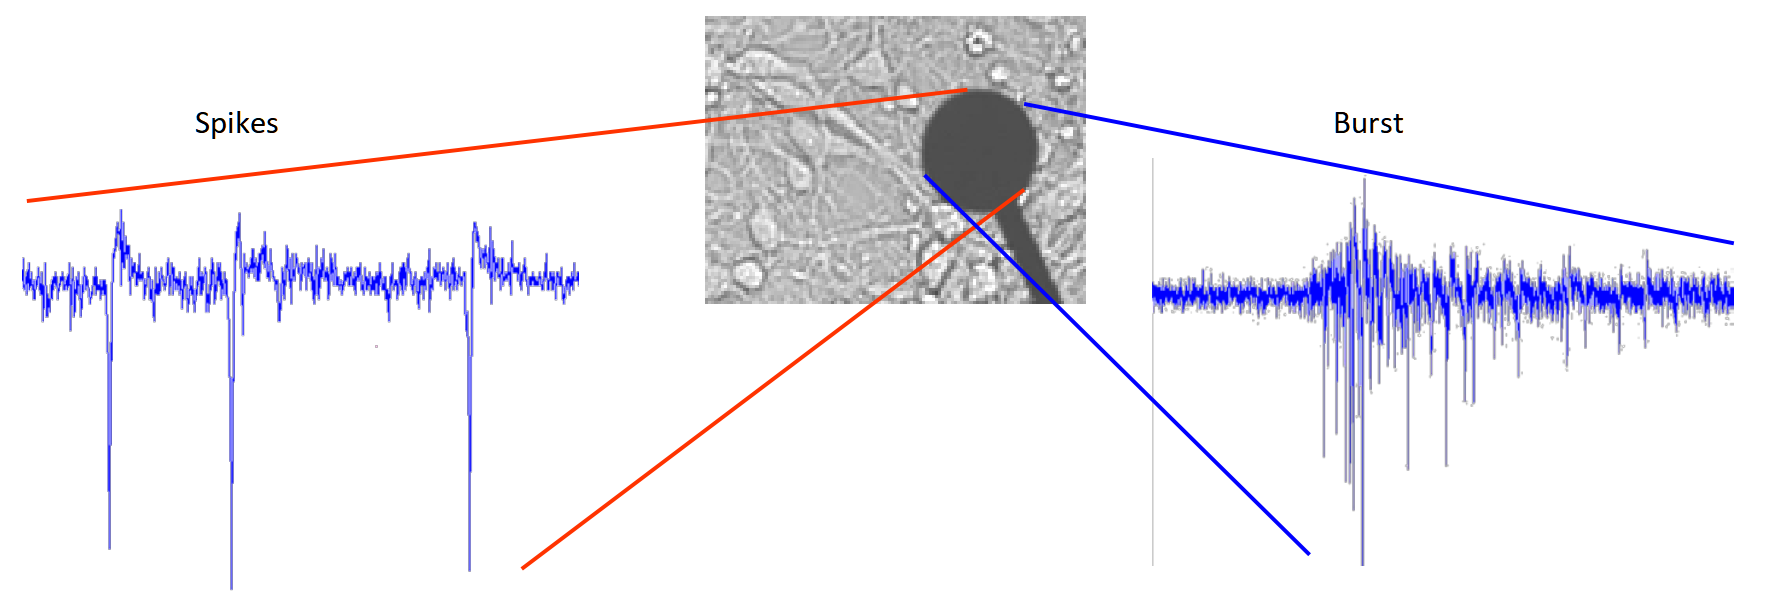
\includegraphics[scale=0.4]{4_1}
    \centering
\end{figure}


\subsection{Data visualization tools}
The first preliminary steps of Spike Analysis consist in taking a look at the raw data, then
deriving the spike train for each channel and visualize it. Therefore, it might be useful to define
a set of proper plots and metrics for data visualization.
\subsubsection{Raw data multi-channel plot}
The following plot shows the activity - i.e. voltage - recorded by 8 distinct electrodes as a
function of time.
\begin{figure}[H]
    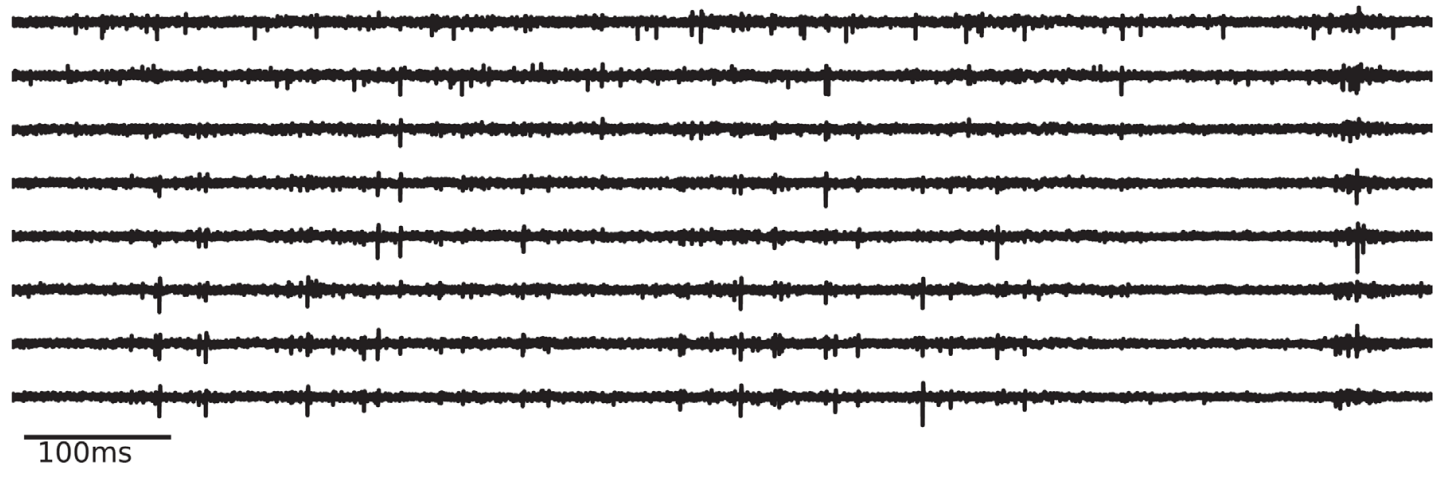
\includegraphics[scale=0.4]{4_2}
    \centering
\end{figure}
\subsubsection{Raster Plot}
The Raster Plot (also known as Spike Raster) is done after Spike Sorting and it allows to visualize
at the same time the spike trains coming from multple recording electrodes on the same time axis.
It is common to observe consistent activation patterns across channels, as neurons influence each
other.
\begin{figure}[H]
    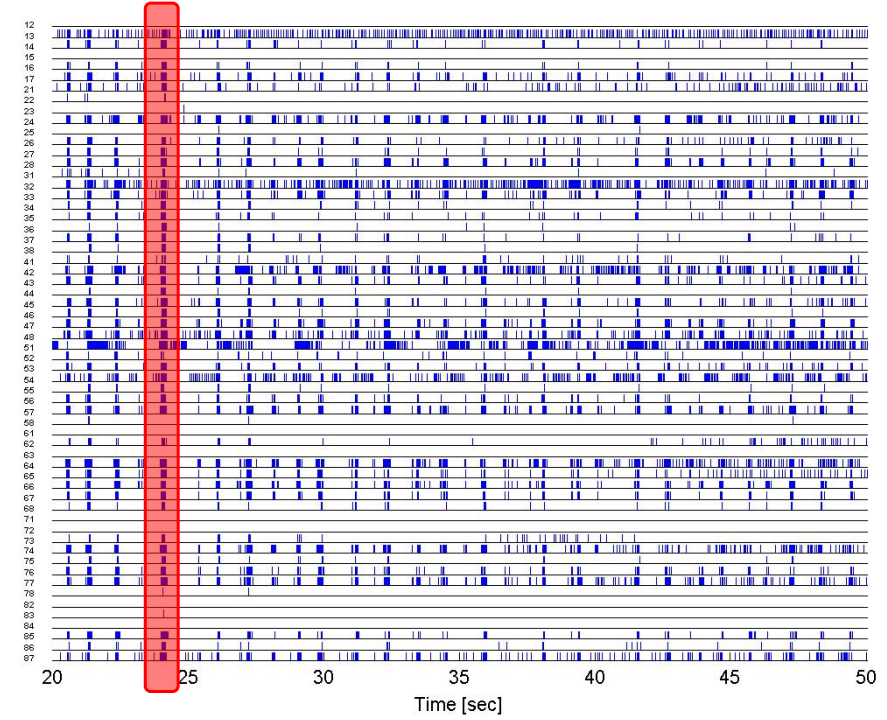
\includegraphics[scale=0.75]{4_3}
    \centering
\end{figure}
\subsubsection{Task-Related Raster Plot}
The Task-Related (or Stimulus-Related) Raster Plot is similar to the ordinary Raster Plot, even if it
has a quite different meaning: the multiple lines do not represent channels, but portions of the
recording coming from just one channel. The signal portions are divided according to the execution of
a task or the receiving of a stimulus.
\begin{figure}[H]
    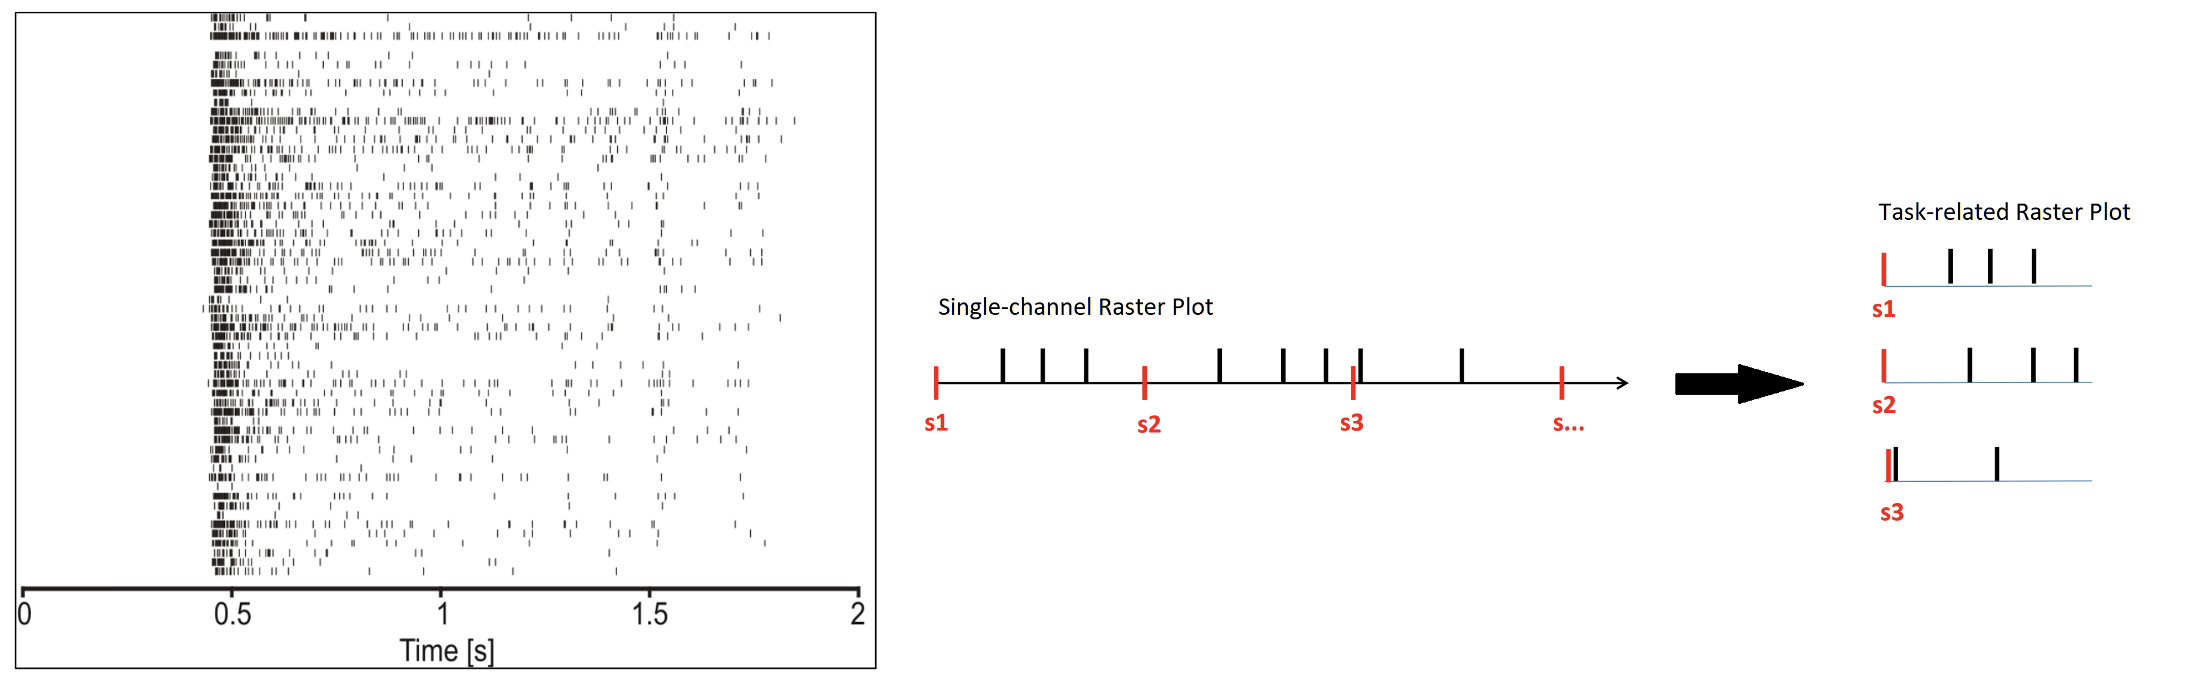
\includegraphics[scale=0.4]{4_4}
    \centering
\end{figure}
\subsubsection{High-Density Data Raster Plot}
This is once again a type of Raster Plot. Data comes from several channels and they cover a relatively
large span of time. As a consequence, it is almost impossible to distinguish single spikes by eye,
thus this high-density plot is usually inspected by looking at the shaded regions, as they exhibit a
higher concentration of fired spikes, implying a greater activity.
\begin{figure}[H]
    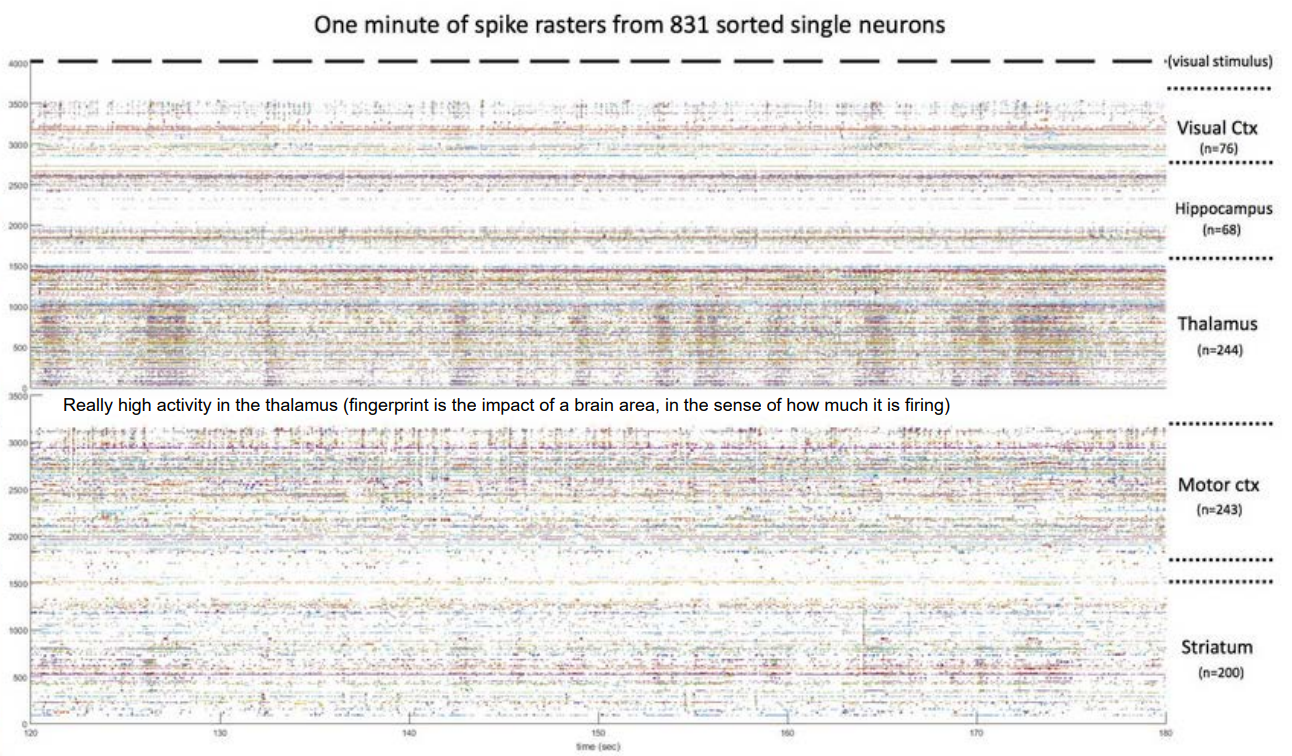
\includegraphics[scale=0.6]{4_5}
    \centering
\end{figure}
\subsubsection{Spike Count and Firing Rate metrics}
\paragraph{Spike Count}
This metric is obtained by dividing the time axis into equal bins \(\Delta{t}=[t_a,t_b]\) and just
counting the number of spikes \(N_{ab}\) occurring in each bin.
Then, an histogram showing the Spike Count can be plotted.
\paragraph{Instantaneous Firing Rate}
By simply taking the Spike Count and dividing it by the bin size, the Instantaneous Firing Rate (IFR)
can be derived.
\begin{align*}
    IFR=r(t)=\frac{N_{ab}(t)}{\Delta{t}}
\end{align*}
The IFR is measured in spikes per second.
\paragraph{Spike Density Function}
The Spike Density Function (SDF) is obtained by associating a proper distribution (typically Gaussian)
to each single spike, then the SDF is derived by summing up the various individual distributions.
\begin{figure}[H]
    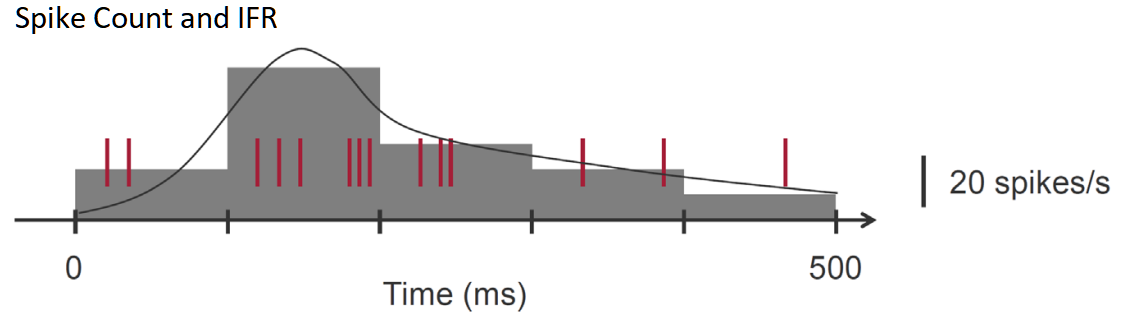
\includegraphics[scale=0.6]{4_6}
    \centering
\end{figure}
\paragraph{Array-Wide Firing Rate}
The Array-Wide Firing Rate (AWFR), often called Average Firing Rate (AFR), it is a sort of
IFR by taking into account the whole network - i.e. all the recorded channles, not just a single one.
This metric is often employed in neuropharmacology, in order to assess the time of response of a drug.\\
By setting the number of channels - i.e. the number of electrodes - to \(M\), the AFR is defined as:
\begin{align*}
    AWFR=awfr(t)=mean(IFR)=\frac{1}{M}\sum_{j=1}^{M}r_{j}(t)
\end{align*}
\paragraph{Mean Firing Rate}
The Mean Firing Rate (MFR) represents a single numerical metric of the activity of neurons for the
entire network (\(M\) channels). It is expressed as
\begin{align*}
    MFR=\frac{1}{T}\sum_{j=1}^{M}N_j
\end{align*}
where \(T\) is the considered time window (somehow corresponding to the previously seen \(\Delta{t}\)),
while \(N_j\) is the number of spikes recorded in the \(T\) interval for the \(j\)-th electrode.\\
Notice once again that both IFR and AWFR are functions of time, continuous in the time-domain, while
MFR is a single value giving information on the average degree of activation of the whole neural
network in a determined time interval.\\
The following plot illustrates the Mean Firing Rate, indicating the average neural activity, at
different concentrations of a brain inhibitor drug.
\begin{figure}[H]
    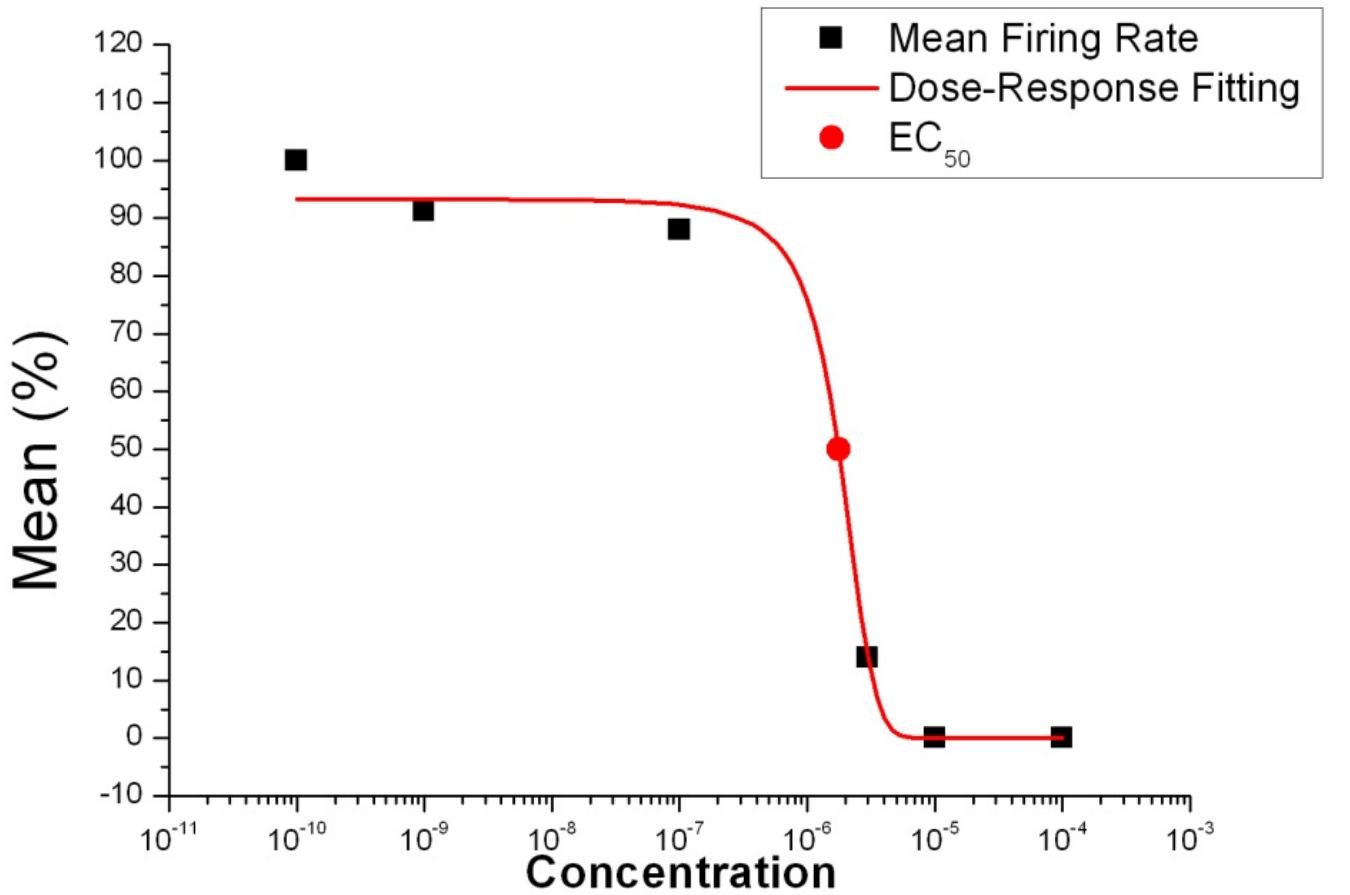
\includegraphics[scale=0.35]{4_7}
    \centering
\end{figure}
\subsubsection{Inter Spike Interval}
\paragraph{Inter Spike Interval}
The Inter Spike Interval (ISI) is the interval between two consecutive spikes. It is used to compute
the Inter Spike Interval Histogram (ISIH), an index of the probability that a spike is fired
a certain time \(\tau\) after a reference spike.
Given \(N\) spikes, the ISIH metric is computed as shown below:
\begin{align*}
    ISIH(\tau)=\frac{1}{N-1}\sum_{s=1}^{N-1}\delta{(t_{s+1}-t_{s}-\tau)}
\end{align*}
An histogram as the following one is often employed to visualize the metric.
\begin{figure}[H]
    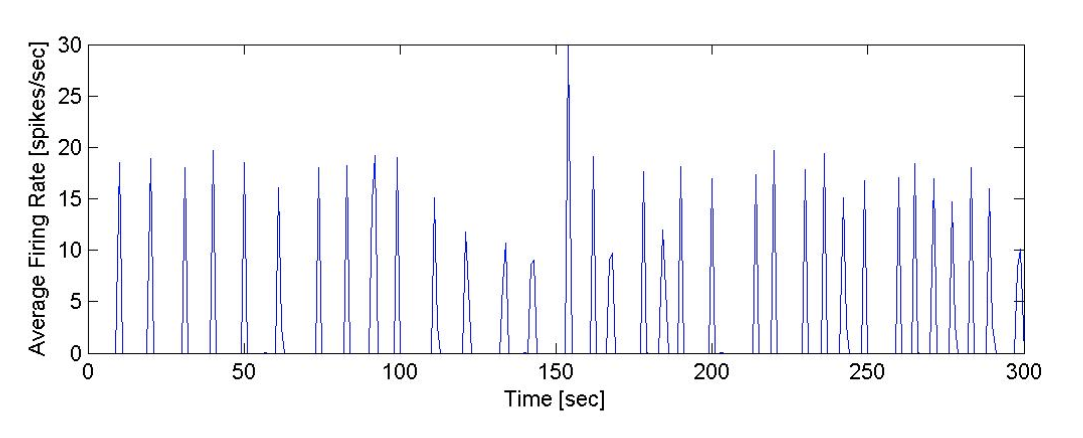
\includegraphics[scale=0.5]{4_8}
    \centering
\end{figure}
Notice that it is common to have a higher probability close to the reference spike, while it tends to
decrease as the Inter Spike Interval grows. If the spike train is made of packed spikes alternating
to empty intervals, then the histogram will display 2 distinct peaks: one for the high frequency
component and one for the low frequency component.
\paragraph{Joint Inter Spike Interval}
The Joint Inter Spike Interval (JISI) is derived from the ISI and it is useful to evaluate the
relationship between pre-ISI and post-ISI intervals, for any spike of the train.
The probability JISIH for \(N\) spikes is computed as:
\begin{align*}
    JISIH(\tau_{post},\tau_{pre})=\frac{1}{N-2}\sum_{s=2}^{N-1}\delta{(t_{s+1}-t_{s}-\tau_{post})}\ast \delta{(t_s-t_{s-1}-\tau_{pre})}
\end{align*}
In this case the plot becomes tridimensional, however it can be displayed in 2D by using
colormaps.
\begin{figure}[H]
    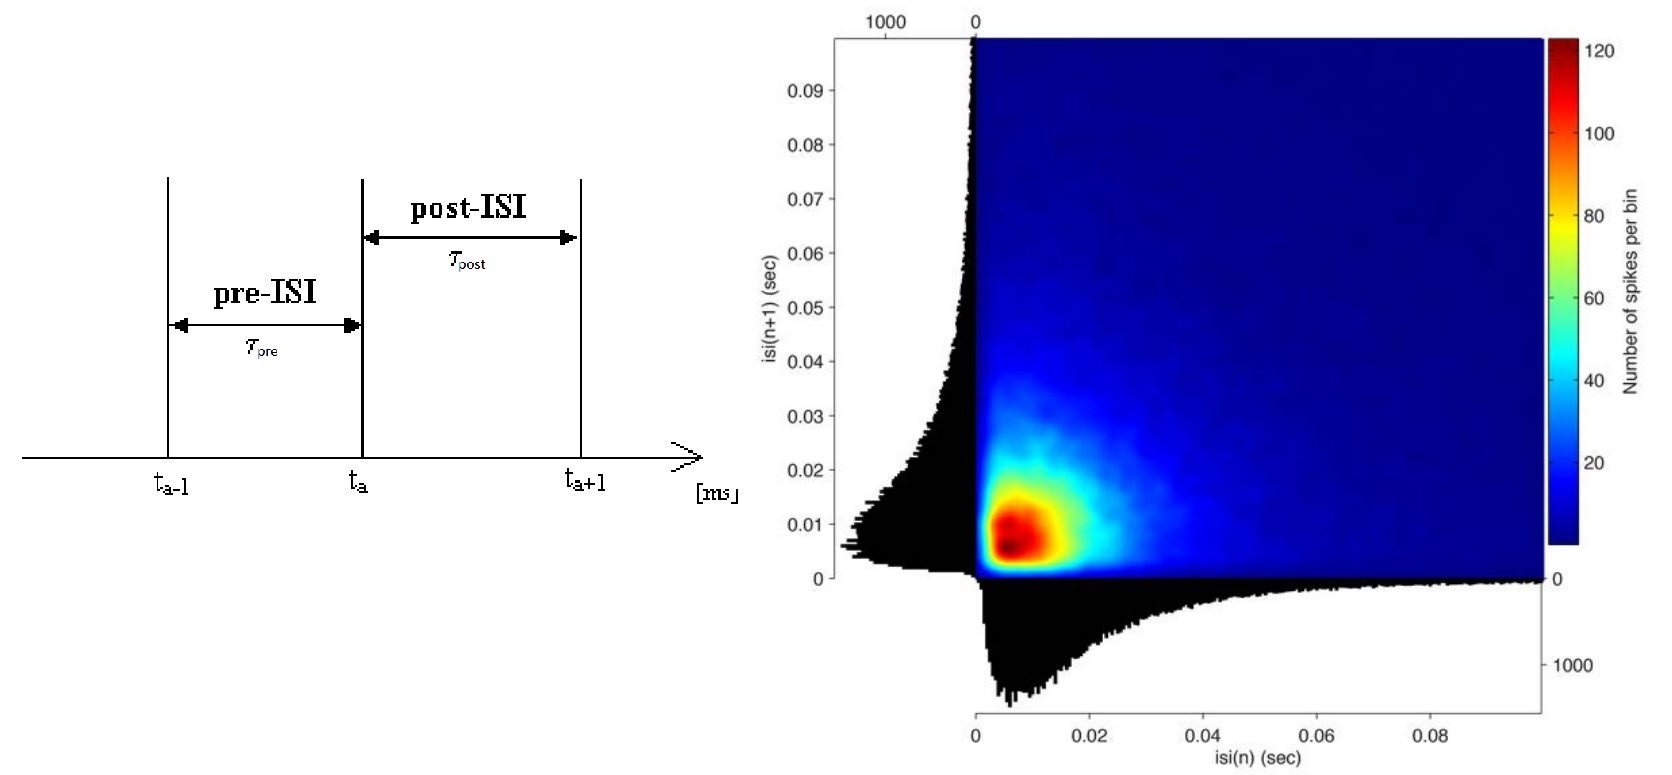
\includegraphics[scale=0.45]{4_9}
    \centering
\end{figure}
\paragraph{Cross Inter Spike Interval}
The Cross Inter Spike Interval (CISI) works in a fashion similar to JISI, but it analyzes the
dependance between spikes of two different trains. The probability CISIH is given by:
\begin{align*}
    CISIH(\tau_{post},\tau_{cross})=\frac{1}{N-2}\sum_{a=1}^{N_a-1}\delta{(t_{a+1}-t_{a}-\tau_{post})}\ast \delta{(t_a-t_b-\tau_{cross})}
\end{align*}
\begin{figure}[H]
    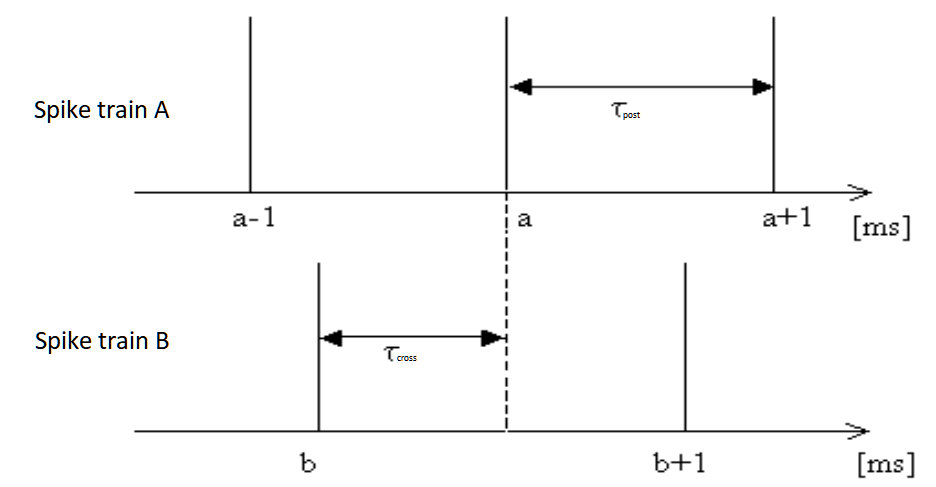
\includegraphics[scale=0.5]{4_10}
    \centering
\end{figure}

\subsection{Spike Generation Modelling}
Several neurons exhibit a considerable degree of variability in their firing
sequence, especially in \textit{in vivo} recordings. Therefore, a class of irregual
spike trains model can be defined after these 3 assumptions:
\begin{enumerate}
    \item Every spike is generated randomly.
    \item Every spike is independent of other spikes.
    \item Every spike has a uniform probability of occurrence in time.
\end{enumerate}
A simple model exploiting the Poisson distribution can be built and it is comparable
to actual spike trains, due to the independence between the time of occurrence of
neighbouring spikes. However, real spike trains tend to have inter spike intervals
(ISI) dependent on the preceding spike intervals.
In general, a Poisson spike sequence is well-suited at describing tonic firing
neurons.
\subsubsection{Derivation of the Homogenous Poisson Process}
Firstly, let's set an assumption: the firing rate - i.e. the average number
of fired spikes in a unit of time - is assumed to be constant, thus
\(r(t)=r=\frac{n}{T}\), where \(n\) is the overall number of observed spikes
and \(T\) is the total observation period.\\
Now, let's divide the observation period \(T\) in a number \(M\) of bins having
equal length, such that \(M=\frac{T}{\Delta{t}}\). Let's consider a
number of bins \(M\) such that every bin contains 1 or 0 spikes. Therefore,
the probability of finding 1 spike in a time interval \(\Delta{t}\) (coincident
with 1 bin) is:
\begin{align*}
    P\{\text{1 spike in}\,\Delta{t}\}=P_{\Delta{t}}[1]
    =\frac{\text{Number of spikes in}\,T}{\text{Number of bins}\,\Delta{t}}
    =\frac{r\cdot{T}}{M}
    =r\cdot\frac{T}{M}
    =r\cdot{\Delta{t}}
\end{align*}
Let's call \(P\{n\,\text{spikes in}\,T\}=P_T[n]\) the probability of finding \(n\)
spikes in the observation period \(T\). It is the product of three distinct factors:
\begin{itemize}
    \item \(P\{\text{Generating}\,n\,\text{spikes within}\,n\,\text{bins}\}
          =\bigl(r\cdot{\Delta{t}}\bigr)^n\)
    \item \(P\{\text{Not generating any spike in the remaining bins}\}
          =\bigl(1-r\cdot{\Delta{t}}\bigr)^{M-n}\)
    \item The number of combinations to put \(n\) spikes in \(M\) bins
          \(\Rightarrow\binom{M}{n}=\frac{M!}{(M-n)!\cdot{n!}}\)
\end{itemize}
Finally, the Poisson model can be written as follow, by recalling the binomial formula:
\begin{align*}
    P=\binom{M}{n}\cdot{p^n}\cdot{q^{M-n}}
\end{align*}
At this point, let's compute the product and try to rearrange it:
\begin{align*}
    P_T[n]=P\{n\,\text{spikes in}\,T\}
     & =\lim_{\Delta{t}\to{0}}\binom{M}{n}\cdot{p^n}\cdot{q^{M-n}}                                                                         \\
     & =\lim_{\Delta{t}\to{0}}\frac{M!}{(M-n)!\cdot{n!}}\cdot{\bigl(r\cdot{\Delta{t}}\bigr)^n}\cdot{\bigl(1-r\cdot{\Delta{t}}\bigr)^{M-n}}
\end{align*}
Let's set \(\epsilon=-r\cdot{\Delta{t}}\Rightarrow \Delta{t}=-\frac{\epsilon}{r}\)
and \(M=\frac{T}{\Delta{t}}=\frac{T}{-\frac{\epsilon}{r}}=-\frac{r\cdot{T}}{\epsilon}\).
For \(\Delta{t}\to{0}\), the number of bins \(M\) becomes larger and larger,
thus \(\bigl(M-n\bigr)\sim{M}=\frac{T}{\Delta{t}}\), leading to:
\begin{align*}
    \lim_{\Delta{t}\to{0}}\bigl(1-r\cdot{\Delta{t}}\bigr)^{M-n}
    \sim\lim_{\Delta{t}\to{0}}\bigl(1-r\cdot{\Delta{t}}\bigr)^M
     & =\lim_{\epsilon\to{0}}\bigl(1+\epsilon\bigr)^M
    =\lim_{\epsilon\to{0}}\bigl(1+\epsilon\bigr)^{-\frac{r\cdot{T}}{\epsilon}}                      \\
     & =\lim_{\epsilon\to{0}}\biggl[\bigl(1+\epsilon\bigr)^{\frac{1}{\epsilon}}\biggr]^{-r\cdot{T}}
    =e^{-r\cdot{T}}
\end{align*}
Let's now consider the binomial coefficient part:
\begin{align*}
    \frac{M!}{(M-n)!\cdot{n!}}
    \sim\frac{M^n}{n!}
    =\frac{\bigl(\frac{T}{\Delta{t}}\bigr)^n}{n!}
    =\frac{T^n}{\Delta{t}^n\cdot{n!}}
\end{align*}
Therefore:
\begin{align*}
    P_T[n]
     & =\lim_{\Delta{t}\to{0}}\frac{M!}{(M-n)!\cdot{n!}}\cdot{\bigl(r\cdot{\Delta{t}}\bigr)^n}\cdot{\bigl(1-r\cdot{\Delta{t}}\bigr)^{M-n}} \\
     & =\frac{T^n}{\Delta{t}^n\cdot{n!}}\cdot{\bigl(r\cdot{\Delta{t}}\bigr)^n}\cdot{e^{-r\cdot{T}}}                                        \\
     & =\frac{T^n}{\cancel{\Delta{t}^n}\cdot{n!}}\cdot{r^n\cdot{\cancel{\Delta{t}^n}}}\cdot{e^{-r\cdot{T}}}                                \\
     & =\frac{\bigl(rT\bigr)^n}{n!}\cdot{e^{-rT}}
\end{align*}
Let's now consider two subsequent time instants \(t_0\) and \(t_0+\tau\), then compute
the following probabilities:
\begin{align*}
    P\{0\,\text{spikes in}\,[t_0,t_0+\tau]\}
    = \frac{\bigl(rT\bigr)^n}{n!}\cdot{e^{-rT}}
    = e^{-rT}
    \quad\quad\quad\text{as \(n=0\)}
\end{align*}
\begin{align*}
    P\{1\,\text{spikes in}\,[t_0,t_0+\tau]\}
    = \frac{\bigl(rT\bigr)^n}{n!}\cdot{e^{-rT}}
    = 1-e^{-rT}
    \quad\quad\quad\text{as \(n=1\)}
\end{align*}
Therefore, the cumulative distribution is 0 for \(\tau=0\) and it increases
monotonically for \(\tau\to{+\infty}\). This means that, after a spiking event,
the longer it is waited, the bigger is the chance for another spike to occur.
At this point, the probability density function describing the waiting times to
have a new spiking event can be expressed as the derivative of the cumulative
distribution:
\begin{align*}
    pdf(\tau)
    =p(\tau)
    =\frac{d}{dt}\bigl(1-e^{-r\tau}\bigr)
    =-(-r)\cdot{e^{-r\tau}}
    =r\cdot{e^{-r\tau}}
\end{align*}
Notice that this last expression represent the distribution of the Inter Spike
Interval (ISI) histogram of a Poisson distribution, with \(\frac{1}{r}\) being
the mean delay between two consecutive events.
Another point to highlight is that the choice of \(t_0\) does not affect the chance
to generate a spike after a time interval \(\tau\).
By chanching the involved variables, the probability density function of a
Poisson distribution, intended as the chance to generate a spike event after a time
\(t\) from a reference spike, is given by
\begin{align*}
    pdf(t)
    =p(t)
    =\frac{1}{\overline{t}}e^{-\frac{t}{\overline{t}}}
\end{align*}
with \(t=\tau\) and \(\frac{1}{\overline{t}}=r=AFR\).\\
In general, the function \(p(t)\) - i.e. the ISI histogram - is obtained
experimentally by binning consecutive inter spike intervals.

\subsubsection{Metrics related to ISI histograms}
\paragraph{Coefficient of Variation}
It is the simplest index to measure the variability of the ISI distribution. The
coefficient of variation \(C_v\) is a dimensionless number computed as the
s.t.d. of the ISI distribution normalized by the mean interspike interval:
\begin{align*}
    C_v=\frac{\sigma_t}{\overline{t}}
\end{align*}
Notice that if the ISI distribution s.t.d. is equal to the mean ISI, then
\(C_v=1\), as in the case of a Poisson distribution. On the other hand,
\(C_v=0\) for a sequence of perfectly regular intervals.

\paragraph{Local Variation}
The previously introduced coefficient of variation \(C_v\) represents the global
variability of an entire ISI sequence, thus it is sensitive to firing rate
fluctuations. Sometimes this might not be enough to discriminate between really
different ISI sequences, as long as they have an equal average firing rate. Hence,
the local variation coefficient \(L_v\) is to be introduced as follow:
\begin{align*}
    L_v
    =\frac{3}{n-1}\sum_{i=1}^{n-1}\biggl(\frac{I_{i}-I_{i+1}}{I_{i}+I_{i+1}}\biggr)^2
    =\frac{3}{n-1}\sum_{i=1}^{n-1}\biggl(1-\frac{4I_{i}I_{i+1}}{(I_{i}+I_{i+1})^2}\biggr)
\end{align*}
This metric is capable to detect also the Instantaneous variability of inter spike
intervals. In other words, the local variation takes into account also the
temporal localization of spikes with respect to one another, not jsut their
average distribution.\\
The following picture is especially useful to emphasize the difference between
\(C_v\) and \(L_v\). The presented spike trains are significantly different from
one another, but their overall distribution is similar. As a result, the
coefficient of variation \(C_v\) is the same, while the local variation \(L_v\)
changes according to the relative distribution of spikes.
\begin{figure}[H]
    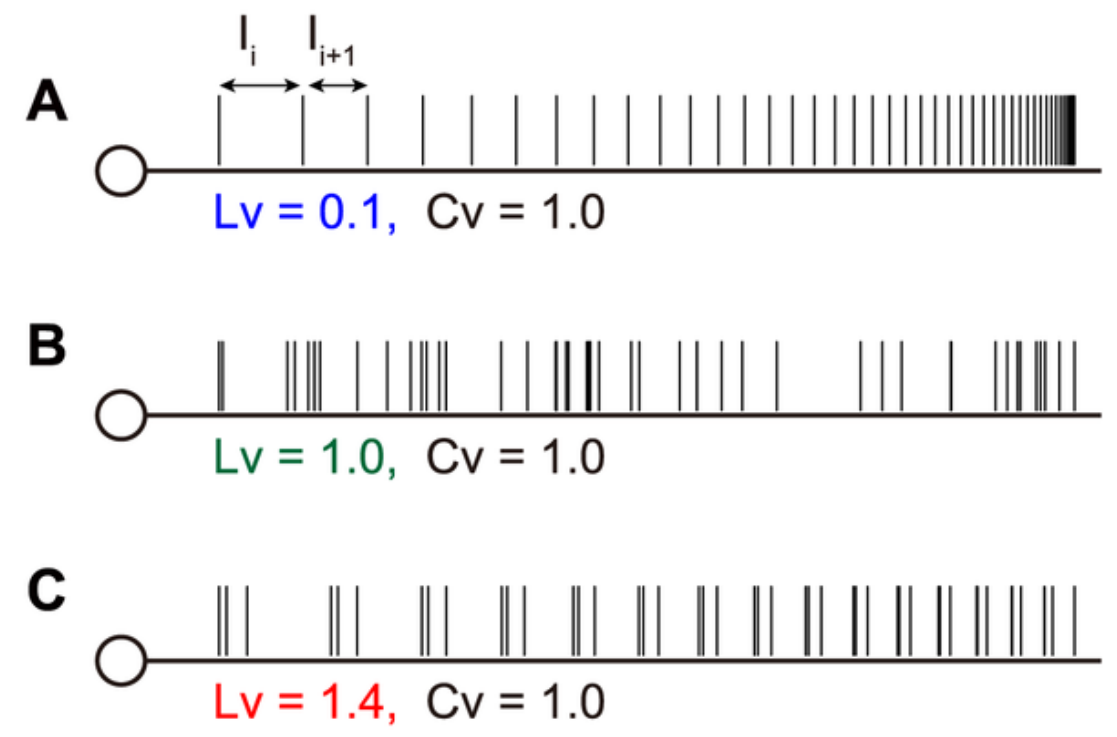
\includegraphics[scale=0.35]{4_11}
    \centering
\end{figure}

\paragraph{LvR}
This metric known as \(L_{v}R\) represents an enhancement with respect to the widely
employed local variation \(L_v\), as a matter of fact it exhibits an enhanced
invariance w.r.t. firing rate fluctuations. It is defined by the expression below:
\begin{align*}
    L_{v}R
    =\frac{3}{n-1}\sum_{i=1}^{n-1}\biggl(1-\frac{4I_{i}I_{i+1}}{(I_{i}+I_{i+1})^2}\biggr)\biggl(1+\frac{4R}{I_{i}+I_{i+1}}\biggr)
\end{align*}
where \(R\) is the refractoriness constant.
This coefficient allows to distinguish among 3 main classes of spike generation,
according to the displacement of spikes with respect to one another:
\begin{itemize}
    \item \(\mathbf{L_{v}R\sim0.5}\Rightarrow\,\)regular pattern
    \item \(\mathbf{L_{v}R\sim1}\Rightarrow\,\)random pattern
    \item \(\mathbf{L_{v}R\sim1.5}\Rightarrow\,\)bursty pattern
\end{itemize}
The image reported in the following shows the previously mentioned 3 spike generation
patterns, in this case employed to identify specific cortical areas.
\begin{figure}[H]
    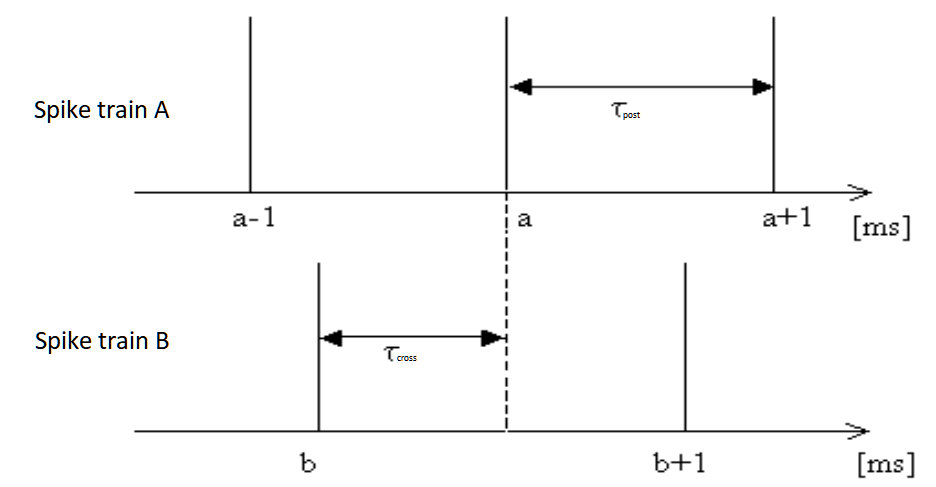
\includegraphics[scale=0.75]{4_12}
    \centering
\end{figure}